\documentclass[a4paper,12pt,oneside]{book}
\usepackage[italian]{babel}
\usepackage[utf8]{inputenc}
\usepackage{textcomp}
\usepackage[parfill]{parskip} %Se necessatrio non indenta, ma inserisce spazio
\usepackage{graphicx}
\usepackage{hyperref}
\usepackage{amsmath} %To number equations

\usepackage{titling}
\newcommand{\subtitle}[1]{%
 \posttitle{%
 \par\end{center}
 \begin{center}\large#1\end{center}
 \vskip6.5em}%
}

\author{Andrea Onofri e Dario Sacco}
\date{Update: v. 0.9 (18/01/2020), compil. 2020-02-04}
\title{Metodologia sperimentale per le scienze agrarie}
\subtitle{}


%***************************************************************

%Specific RMarkdown
\usepackage{color}
\usepackage{fancyvrb}
\usepackage{longtable}
\usepackage{booktabs}
\providecommand{\tightlist}{%
  \setlength{\itemsep}{0pt}\setlength{\parskip}{0pt}}
\newcommand{\VerbBar}{|}
\newcommand{\VERB}{\Verb[commandchars=\\\{\}]}
\DefineVerbatimEnvironment{Highlighting}{Verbatim}{commandchars=\\\{\},fontsize=\small}
\usepackage{framed}
\newenvironment{Shaded}{}{}
\definecolor{shadecolor}{RGB}{250,248,248}
\newcommand{\KeywordTok}[1]{#1}
\newcommand{\DataTypeTok}[1]{#1}
\newcommand{\DecValTok}[1]{#1}
\newcommand{\BaseNTok}[1]{#1}
\newcommand{\FloatTok}[1]{#1}
\newcommand{\ConstantTok}[1]{#1}
\newcommand{\CharTok}[1]{#1}
\newcommand{\SpecialCharTok}[1]{#1}
\newcommand{\StringTok}[1]{#1}
\newcommand{\VerbatimStringTok}[1]{#1}
\newcommand{\SpecialStringTok}[1]{#1}
\newcommand{\ImportTok}[1]{#1}
\newcommand{\CommentTok}[1]{#1}
\newcommand{\DocumentationTok}[1]{#1}
\newcommand{\AnnotationTok}[1]{#1}
\newcommand{\CommentVarTok}[1]{#1}
\newcommand{\OtherTok}[1]{#1}
\newcommand{\FunctionTok}[1]{#1}
\newcommand{\VariableTok}[1]{#1}
\newcommand{\ControlFlowTok}[1]{#1}
\newcommand{\OperatorTok}[1]{#1}
\newcommand{\BuiltInTok}[1]{#1}
\newcommand{\ExtensionTok}[1]{#1}
\newcommand{\PreprocessorTok}[1]{#1}
\newcommand{\AttributeTok}[1]{#1}
\newcommand{\RegionMarkerTok}[1]{#1}
\newcommand{\InformationTok}[1]{#1}
\newcommand{\WarningTok}[1]{#1}
\newcommand{\AlertTok}[1]{#1}
\newcommand{\ErrorTok}[1]{#1}
\newcommand{\NormalTok}[1]{#1}
% Redefine \includegraphics so that, unless explicit options are
% given, the image width will not exceed the width of the page.
% Images get their normal width if they fit onto the page, but
% are scaled down if they would overflow the margins.

\begin{document}

\maketitle
\tableofcontents

\hypertarget{introduzione}{%
\chapter*{Introduzione}\label{introduzione}}
\addcontentsline{toc}{chapter}{Introduzione}

Placeholder

\hypertarget{organizzazione-del-testo}{%
\section*{Organizzazione del testo}\label{organizzazione-del-testo}}
\addcontentsline{toc}{section}{Organizzazione del testo}

\hypertarget{gli-autori}{%
\section*{Gli autori}\label{gli-autori}}
\addcontentsline{toc}{section}{Gli autori}

\hypertarget{pre-requisiti}{%
\section*{Pre-requisiti}\label{pre-requisiti}}
\addcontentsline{toc}{section}{Pre-requisiti}

\hypertarget{packages-aggiuntivi}{%
\section*{Packages aggiuntivi}\label{packages-aggiuntivi}}
\addcontentsline{toc}{section}{Packages aggiuntivi}

\hypertarget{scienza-e-pseudo-scienza}{%
\chapter{Scienza e pseudo-scienza}\label{scienza-e-pseudo-scienza}}

Placeholder

\hypertarget{scienza-dati}{%
\section{Scienza = dati}\label{scienza-dati}}

\hypertarget{dati-buoni-e-cattivi}{%
\section{Dati `buoni' e `cattivi'}\label{dati-buoni-e-cattivi}}

\hypertarget{lerrore-sperimentale}{%
\subsection{L'errore sperimentale}\label{lerrore-sperimentale}}

\hypertarget{la-variabilita-naturale}{%
\subsection{La variabilità naturale}\label{la-variabilita-naturale}}

\hypertarget{il-campionamento}{%
\subsection{Il campionamento}\label{il-campionamento}}

\hypertarget{scienza-metodo}{%
\section{Scienza = metodo}\label{scienza-metodo}}

\hypertarget{elementi-fondamentali-del-disegno-sperimentale}{%
\section{Elementi fondamentali del disegno sperimentale}\label{elementi-fondamentali-del-disegno-sperimentale}}

\hypertarget{controllo-degli-errori}{%
\subsection{Controllo degli errori}\label{controllo-degli-errori}}

\hypertarget{replicazione}{%
\subsection{Replicazione}\label{replicazione}}

\hypertarget{randomizzazione}{%
\subsection{Randomizzazione}\label{randomizzazione}}

\hypertarget{esperimenti-invalidi}{%
\subsection{Esperimenti invalidi}\label{esperimenti-invalidi}}

\hypertarget{cattivo-controllo-degli-errori}{%
\subsubsection{Cattivo controllo degli errori}\label{cattivo-controllo-degli-errori}}

\hypertarget{confounding-e-correlazione-spuria}{%
\subsubsection{`Confounding' e correlazione spuria}\label{confounding-e-correlazione-spuria}}

\hypertarget{pseudo-repliche-e-randomizzazione-poco-attenta}{%
\subsubsection{Pseudo-repliche e randomizzazione poco attenta}\label{pseudo-repliche-e-randomizzazione-poco-attenta}}

\hypertarget{scienza-e-falsificabilita}{%
\section{Scienza e falsificabilità}\label{scienza-e-falsificabilita}}

\hypertarget{chi-valuta-se-un-esperimento-e-attendibile}{%
\section{Chi valuta se un esperimento è attendibile?}\label{chi-valuta-se-un-esperimento-e-attendibile}}

\hypertarget{conclusioni}{%
\section{Conclusioni}\label{conclusioni}}

\hypertarget{per-approfondire-un-po}{%
\section{Per approfondire un po'\ldots{}}\label{per-approfondire-un-po}}

\hypertarget{progettare-un-esperimento}{%
\chapter{Progettare un esperimento}\label{progettare-un-esperimento}}

Qualunque sia l'ambito scientifico, nella progettazione di un esperimento possiamo individuare alcune fasi fondamentali, che proviamo ad elencare:

\begin{enumerate}
\def\labelenumi{\arabic{enumi}.}
\tightlist
\item
  individuazione del background (ricerca bibliografica)
\item
  definizione dell'ipotesi scientifica e dell'obiettivo;
\item
  identificazione dei fattore/i sperimentale/i;
\item
  identificazione dei soggetti sperimentali e delle repliche;
\item
  identificazione delle variabili da rilevare;
\item
  allocazione dei trattamenti;
\item
  impianto dell'esperimento.
\end{enumerate}

Nell'analizzare questi aspetti, faremo riferimento ad alcuni esempi pratici, che verranno presentati tra poco.

\hypertarget{ipotesi-scientifica-rightarrow-obiettivo-dellesperimento}{%
\section{\texorpdfstring{Ipotesi scientifica \(\rightarrow\) obiettivo dell'esperimento}{Ipotesi scientifica \textbackslash{}rightarrow obiettivo dell'esperimento}}\label{ipotesi-scientifica-rightarrow-obiettivo-dellesperimento}}

Trascurando la parte di ricerca bibliografica, che è pur fondamentale, nel metodo scientifico galileiano, il punto di partenza di un esperimento è l'\textbf{ipotesi scientifica}, che determina l'obiettivo dell'esperimento. Si tratta del passaggio fondamentale dal quale dipende in modo logico tutto il lavoro successivo. Gli obiettivi debbono essere:

\begin{enumerate}
\def\labelenumi{\arabic{enumi}.}
\tightlist
\item
  rilevanti;
\item
  chiaramente definiti;
\item
  specifici;
\item
  misurabili;
\item
  raggiungibili/realistici;
\item
  temporalmente organizzati.
\end{enumerate}

Il rischio che si corre con obiettivi mal posti è quello di eseguire una ricerca dispersiva, con raccolta di dati non necessari e/o mancanza di dati fondamentali, con costi più elevati del necessario e un uso poco efficiente delle risorse. In genere, prima si definisce un obiettivo generale, seguito da uno o più obiettivi specifici, in genere proiettati su un più breve spazio temporale e che possono essere visti anche come le fasi necessarie per raggiungere l'obiettivo generale.

\hypertarget{identificazione-dei-fattori-sperimentali}{%
\section{Identificazione dei fattori sperimentali}\label{identificazione-dei-fattori-sperimentali}}

A differeza degli esperimenti \textbf{osservazionali}, più tipici delle scienze naturali, dove ci si limita ad osservare quanto accade in natura, nelle scienze agrarie si tende lavorare con esperimenti manipolati, dove cioè le unità sperimentali sono sottoposte a stimoli differenti a seconda della risposta che si vuole valutare.
Dopo aver definito l'obiettivo di un esperimento, pertanto, è necessario chiarire esattamente gli stimoli a cui saranno sottoposte le unità sperimentali. Uno `stimolo' sperimentale prende il nome di \textbf{fattore sperimentale}, che può avere più \textbf{livelli}. I livelli del fattore sperimentale prendono il nome di \textbf{trattamenti (o tesi) sperimentali}.

\hypertarget{esperimenti-multifattoriali}{%
\subsection{Esperimenti (multi)fattoriali}\label{esperimenti-multifattoriali}}

In alcuni casi è necessario inserire in prova più di un fattore sperimentale. In questo caso si parla di esperimenti \textbf{fattoriali}, che possono essere \textbf{incrociati (crossed)} quando sono presenti in prova tutte le possibili combinazioni dei livelli di ogni fattore, oppure di esperimenti \textbf{innestati (nested)} quando i livelli di un fattore cambiano al cambiare dei livelli dell'altro. Il vantaggio di questi tipi di esperimento è che permettono di valutare non solo l'effetto di ogni singolo fattore, ma anche la risposta congiunta di due fattori, che a volte può essere più che additiva (i due trattamenti insieme permettono un risultato superiore al vantaggio derivante singolarmente dai due trattamenti) o meno che additiva (i due trattamenti in quanche modo si elidono).

Ad esempio:

\begin{enumerate}
\def\labelenumi{\arabic{enumi}.}
\tightlist
\item
  Immaginiamo di voler studiare due fattori sperimentali: la varietà di girasole (tre livelli: A, B e C) e la concimazione (2 livelli: pollino e urea). Abbiamo quindi 6 possibili trattamenti (combinazioni): A-pollina, A-urea, B-pollina, B-urea, C-pollina e C-urea. Il disegno è completamente incrociato.
\item
  Immaginiamo di voler confrontare due specie in agricoltura biologica (orzo e triticale), con tre varietà ciascuna (A, B e C per orzo, D, E e F per triticale). Anche in questo caso abbiamo sei trattamenti: orzo-A, orzo-B, orzo-C, triticale-D, triticale-E e triticale-F, ma il disegno è innestato, perché per il fattore sperimentale `varietà' i livelli cambiano a seconda dei livelli del fattore `specie'.
\end{enumerate}

\hypertarget{limportanza-del-controllo}{%
\subsection{L'importanza del controllo}\label{limportanza-del-controllo}}

In alcuni casi si pone il problema di inserire in prova un trattamento che funga da riferimento per tutti gli altri. In questi casi si parla comunemente di \textbf{controllo} o \textbf{testimone}, che può essere

\begin{enumerate}
\def\labelenumi{\arabic{enumi}.}
\tightlist
\item
  non sottoposto a trattamento
\item
  trattato con placebo
\item
  trattato secondo le modalità usuali di riferimento
\end{enumerate}

Ad esempio, è usuale includere in un confronto varietale, la varietà di riferimento, che ci consente di capire se le prestazione delle nuove varietà sono effettivamente interessanti oppure no.

Per quello che riguarda invece gli studi tossicologici, è evidente l'importanza di includere un controllo non trattato. Il placebo è una preparazione che contiene tutti gli ingredienti della formulazione attiva, meno che il principio attivo. Il placebo si rende necessario in una serie di circostanze, ad esempio:

\begin{enumerate}
\def\labelenumi{\arabic{enumi}.}
\tightlist
\item
  quando il soggetto è influenzabile e può reagire alla semplice idea di essere stato trattato (effetto placebo)
\item
  quando i co-formulanti o la soluzione impiegata per veicolare il principio attivo possono mostrare un effetto sul soggetto.
\end{enumerate}

Poichè gli esperimenti ci permettono non solo di capire se il comportamento di un livello di un fattore è uguale o differente da un altro, ma anche di misurare l'incremento che possiamo avere rispetto ad un altro, è molto importante il ruolo del controllo, perchè esso diventa il riferimento rispetto al quale noi possiamo misurare il miglioramento dell'innovazione testata (`trattato').

\hypertarget{fattori-sperimentali-di-trattamento-e-di-blocco}{%
\subsection{Fattori sperimentali di trattamento e di blocco}\label{fattori-sperimentali-di-trattamento-e-di-blocco}}

Finora abbiamo menzionato quelli che, in lingua inglese, vengono definiti \emph{treatment factor} (trattamenti sperimentali). Tuttavia, possono esserci altri fattori sperimentali non allocati, ma `innati' e legati alla collocazione spazio-temporale o alle caratteristiche dei soggetti. Questi fattori vengono definiti, sempre in inglese, \emph{blocking factors}. Di questi fanno parte, ad esempio, il blocco, la località ed ogni altro elemento che permette di raggruppare i soggetti. Anche questi \emph{blocking factors} devono essere chiaramente identificati ed elencati.

\hypertarget{identificazione-delle-unita-sperimentali}{%
\section{Identificazione delle unità sperimentali}\label{identificazione-delle-unita-sperimentali}}

\hypertarget{cornice-di-campionamento}{%
\subsection{Cornice di campionamento}\label{cornice-di-campionamento}}

Prima di iniziare un esperimento, deve essere chiaro qual è la popolazione di riferimento (cornice di campionamento). Ad esempio, se vogliamo determinare la produttività delle varietà di tabacco e la loro adattabilità alle condizioni umbre, la cornice di campionamento sarà la media e alta valle del Tevere. Se invece vogliamo individuare la risposta di bovini adulti ad un certo tipo di alimentazione, dovremo campionare soggetti di entrambi i sessi, diverse età (ma comunque adulti) e in buone condizioni di salute. Insomma, la cornice di campionamento deve essere composta da soggetti che presentano tutte le caratteristiche richieste dall'obiettivo dell'esperimento.

La scelta della cornice di campionamento è fondamentale, perché è ad essa che si riferiscono i risultati ottenuti; ad esempio, se la cornice di campionamento è la media valle del Tevere, i risultati ottenuti non potranno essere riferiti alla Pianura Padana oppure al Tavoliere delle Puglie.

\hypertarget{scelta-delle-unita-sperimentali}{%
\subsection{Scelta delle unità sperimentali}\label{scelta-delle-unita-sperimentali}}

All'interno della cornice di campionamento, adottando criteri rigorosi, andremo a scegliere i soggetti da includere in prova. I soggetti dovranno essere rappresentativi della cornice di campionamento, ma, per il resto, il più possibile omogenei, per minimizzare le fluttuazioni casuali di rispsposta.

Per quanto riguarda la sperimentazione di pieno campo, l'omogeneità dell'ambiente è fondamentale per aumentare la precisione dell'esperimento, cosa che si consegue, innanzitutto, con la scelta dell'appezzamento giusto. Questa scelta è particolarmente delicata ed è guidata soprattutto dall'esperienza, tenendo conto anche di aspetti come la facilità di accesso e la vicinanza di strutture (laboratori, capannoni\ldots{}), che consentano un'accurata esecuzione degli eventuali prelievi. Oltre a scegliere correttamente l'appezzamento, è importante anche porre in atto alcune operazioni che consentano di incrementare ulteriormente l'omogenità dell'appezzamento prescelto. Ad esempio, talvolta si usa far precedere la prova da una coltura di `omogeneizzazione', ad esempio avena, che è molto avida di azoto e lascia nel terreno poca fertilità residua. Oppure un prato di erba medica, che, grazie agli sfalci periodici, lascia il terreno libero da piante infestanti.

Gli sforzi operati al fine di rendere il più omogeneo possibile l'insieme delle unità sperimentali servono ad aumentare la capacità di rendere evidente l'effetto dei trattamenti praticati. Occorre tuttavia sottolineare che la variabilità è intrinseca nel sistema biologico e questa variabilità diventa il metro di giudizio per verificare se esiste veramente un effetto trattamento o no. Occorre pertanto assicirarsi che l'attività sperimentale non introduca (o introduca il meno possibile) ulteriore variabilità a quella normalmente presente in natura.

\hypertarget{unita-sperimentali-in-campo-le-parcelle}{%
\subsection{Unità sperimentali in campo: le parcelle}\label{unita-sperimentali-in-campo-le-parcelle}}

Solitamente, nella ricerca biologica, le unità sperimentali sono chiaramente definite: un animale, una persona, un insetto, un'aliquota di terreno. In genere, qualunque esse siano, debbono essere chiaramente identificate prima di procedere all'allocazione dei trattamenti.

Nella sperimentazione di pieno campo, le unità sperimentali sono costituite dalle cosiddette `parcelle' (Figura \ref{fig:figName21} ), che, almeno inizialmente, non sono chiaramente identificate. La loro identificazione, dopo aver selezionato l'appezzamento giusto e averlo reso più uniforme possibile, viene usualmente eseguita su carta, redigendo la \textbf{mappa dell'esperimento}.

\begin{figure}

{\centering 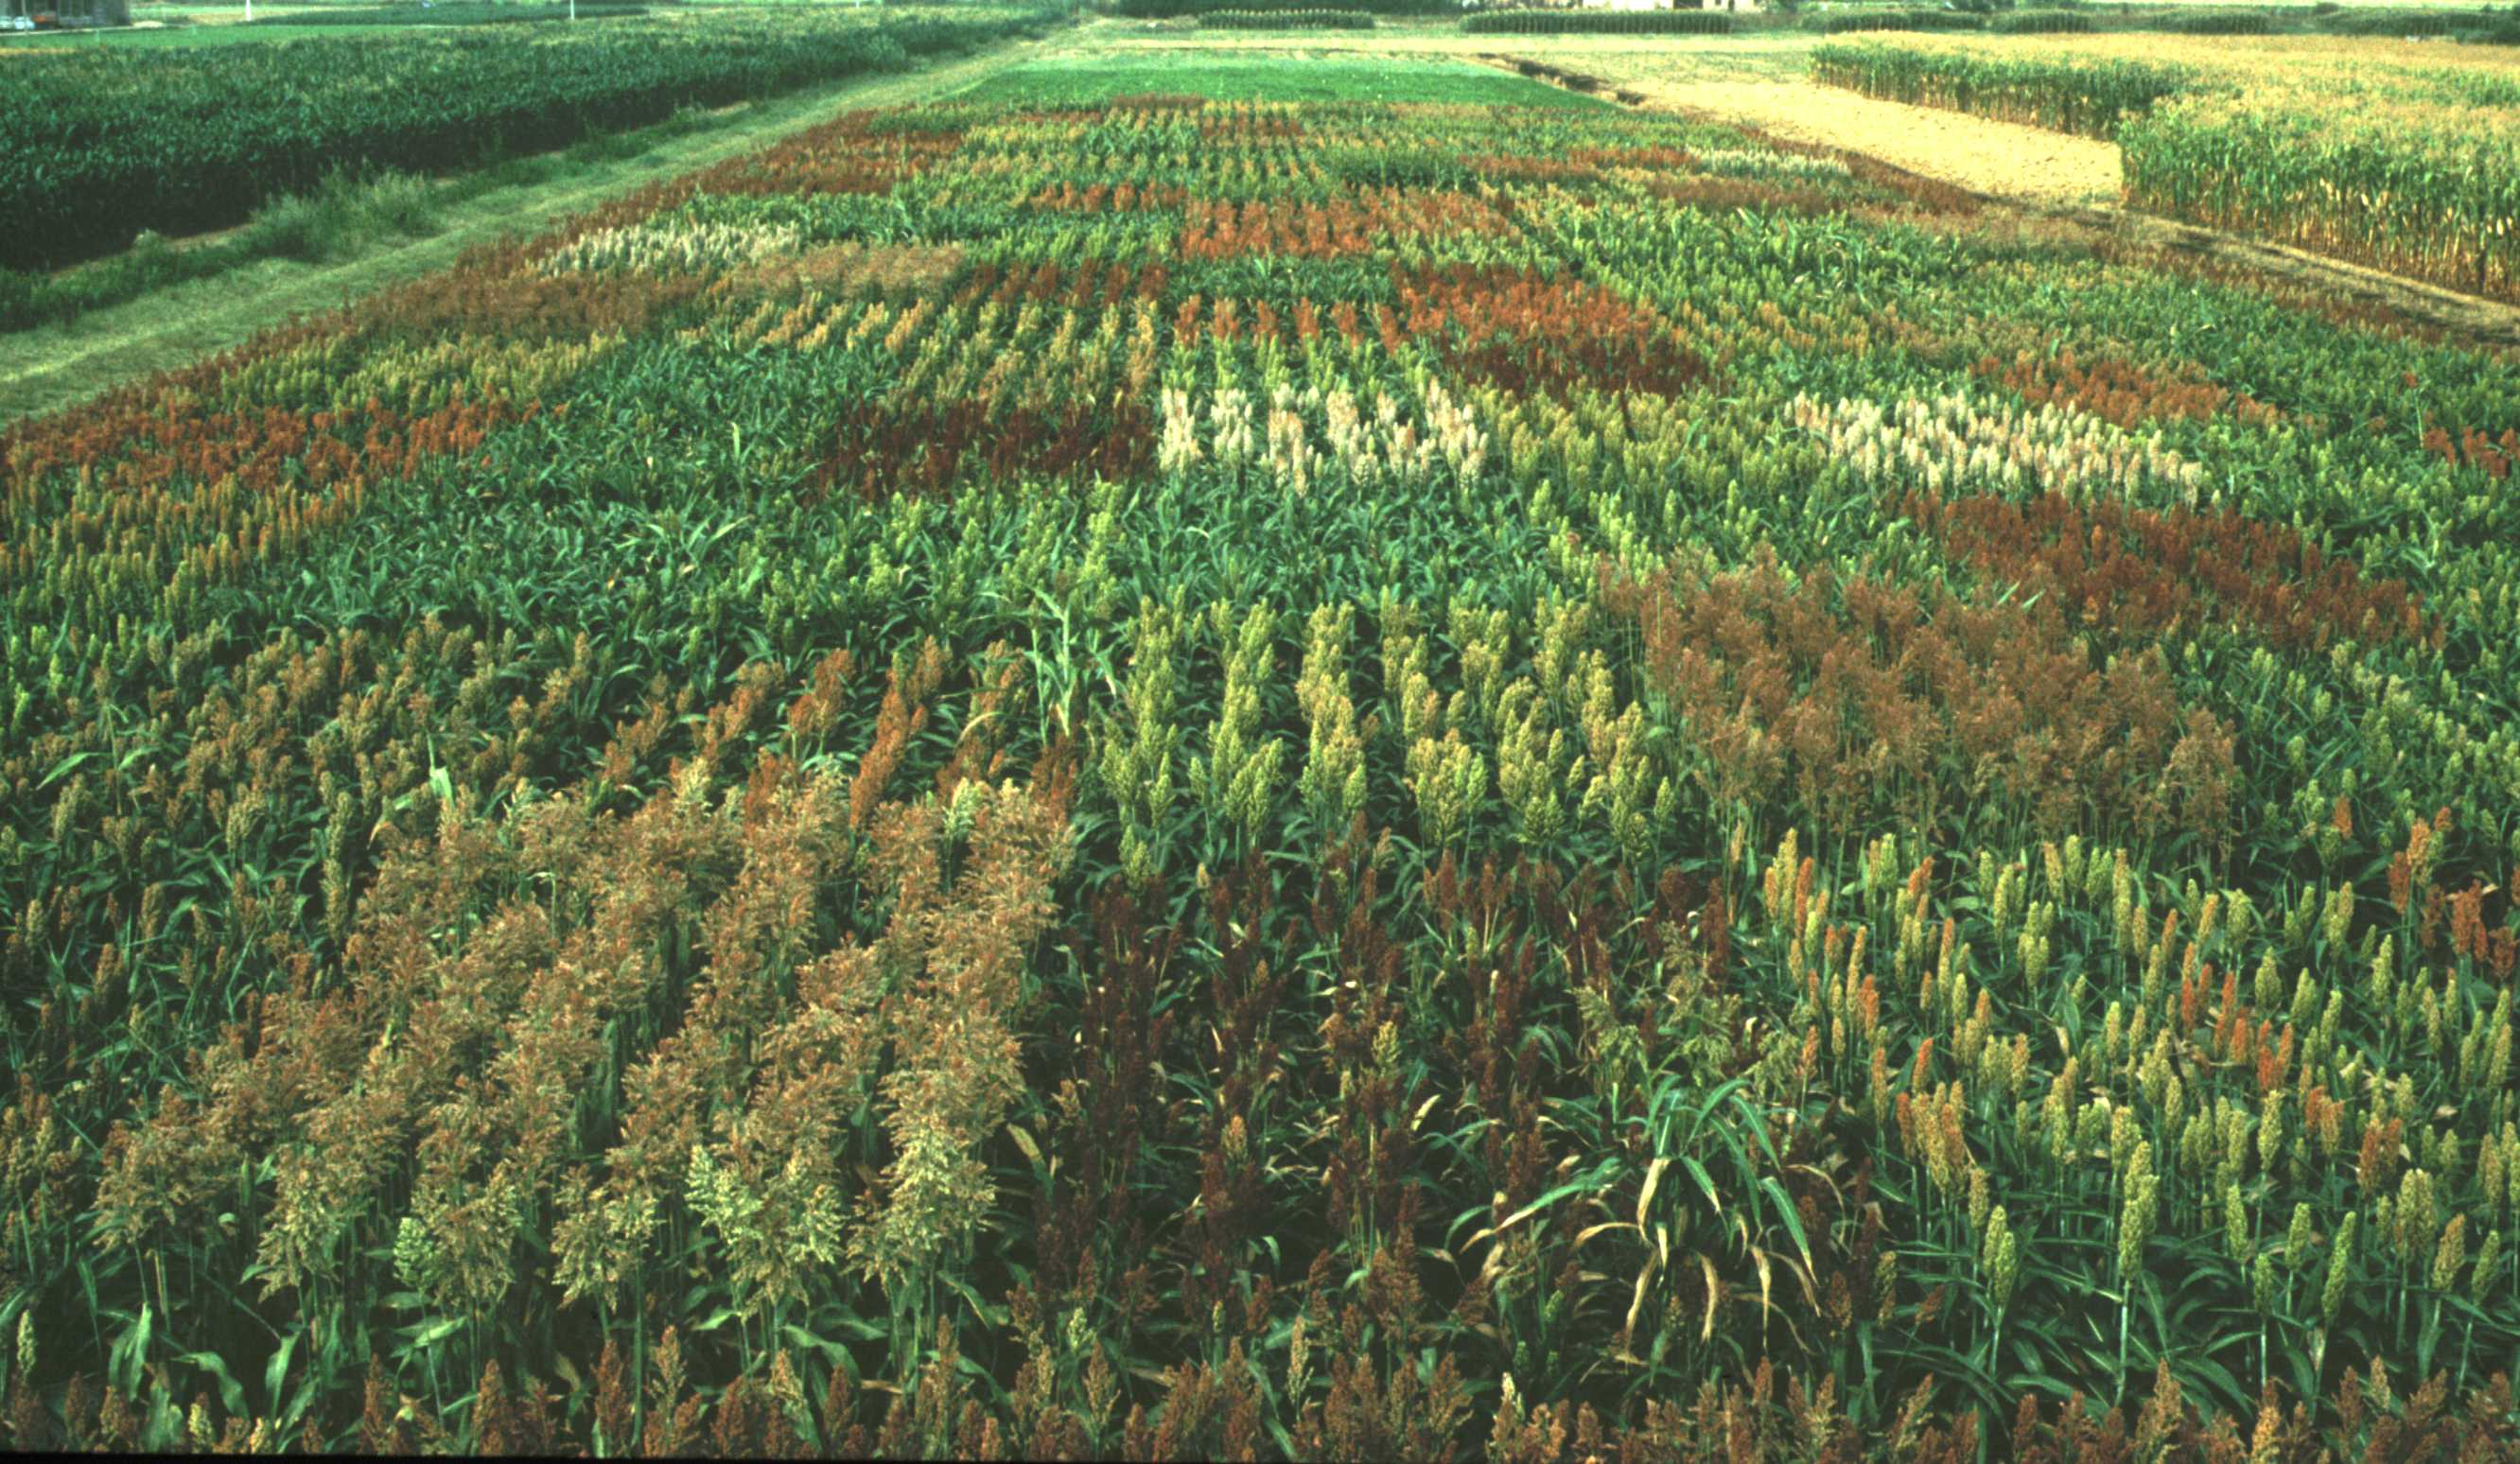
\includegraphics[width=0.9\linewidth]{_images/SorgoProveVarietali} 

}

\caption{Una prova sperimentale in campo (Foto D. Alberati)}\label{fig:figName21}
\end{figure}

In primo luogo, si decide la \textbf{dimensione e la forma della parcella}. L'aspetto fondamentale è che ogni parcella deve contenere un numero di piante sufficientemente alto da essere rappresentativo. Per questo motivo le colture a bassa fittezza (es. mais) hanno sempre bisogno di parcelle più grandi che non quelle ad alta fittezza (es. frumento). La dimensione non deve tuttavia eccedere una certa soglia, in quanto con essa aumenta anche la variabilità del terreno e, di conseguenza, diminuisce l'omogeneità dell'esperimento. Per questo motivo, talvolta si preferisce diminuire la dimensione delle parcelle ed, avendo lo spazio sufficiente, aumentare il numero delle repliche. E' poi importante tenere conto di come saranno effettuare le pratiche colturali. Se queste saranno effettuate con normali attrezzature aziendali, occorre tenere conto della larghezza di lavoro degli organi lavoranti ed utilizzare multipli di questi.

Nello stabilire la dimensione delle parcelle, dovremo tener conto del fatto che la parte più delicata è il bordo, in quanto le piante che si trovano lungo il bordo esterno risentono di condizioni diverse dalle altre piante situate al centro della parcella (\textbf{effetto bordo}). Questo determina variabilità all'interno della parcella, che possiamo minimizzare raccogliendo solo la parte centrale. Si viene così a distinguere la superficie totale della parcella dalla superficie di raccolta (\textbf{superficie utile}), che può essere anche molto minore di quella totale.

Tenendo conto degli aspetti detti in precedenza, ritieniamo che le colture ad elevata fittezza (frumento, cereali, erba medica\ldots{}) dovrebbero avere parcelle di almeno 10-20 m\textsuperscript{2}, mentre a bassa fittezza (mais, girasole\ldots{}) dovrebbero avere parcelle di almeno 20-40 m\textsuperscript{2}. Queste dimensioni sono riferite alla superficie utile di raccolta, non alla dimensione totale: se si ritiene di dover raccogliere solo una parte della parcella per limitare l'effetto bordo, allora le dimensioni totali dovranno essere opportunamente aumentate, rispetto a quanto indicato sopra.

Per quanto riguarda la forma, le parcelle quadrate minimizzano l'effetto bordo, perché, a parità di superficie, hanno un perimetro più basso. Tuttavia esse sono di più difficile gestione, in quanto, considerando il fronte di lavoro di una seminatrice o una mietitrebbiatrice parcellare, possono richiedere la semina o la raccolta in più passate, il che finisce per essere una fonte di errore. Per questo motivo le parcelle sono usualmente rettangolari, con una larghezza pari a quella delle macchine operatrici.

Dopo aver stabilito la forma e la dimensione delle parcelle, si può procedere alla redazione della mappa, tenendo conto che il numero delle parcelle risulta dal prodotto tra il numero delle tesi sperimentali e il numero delle repliche.

In genere, si cerca di fare in modo che l'esperimento no sia troppo lungo (il che potrebbe aumenterebbe la variabilità), ma neanche troppo largo, per evitare di avvicinarsi troppo alle scoline, dove possono manifestarsi ristagni idrici. Lungo il contorno della prova è possibile sistemare altre parcelle fuori esperimento con funzione di `bordi'. In questo modo si evita che i bordi esterni delle parcelle esterne siano esposti a condizioni molto diverse dagli altri, cosa che potrebbe accentuare l'effetto `bordo', di cui abbiamo parlato in precedenza. Queste parcelle di bordo verranno trattate in modo ordinario.

La figura \ref{fig:figName31} riporta la mappa di un esperimento sistemato su un appezzamento largo 30 metri e lungo 400 metri. In questo caso abbiamo disegnato otto file di parcelle in senso trasversale (8 x 2.25 m = 18 m di larghezza), e quattro parcelle in senso longitudinale. Vediamo in figura che la mappa riporta tutte le informazioni relative al disegno sperimentale in modo da facilitare l'orientamento della mappa stessa. Un altro fondamentale aspetto è che le parcelle sono tutte chiaramente identificate con un numero.

\begin{figure}

{\centering 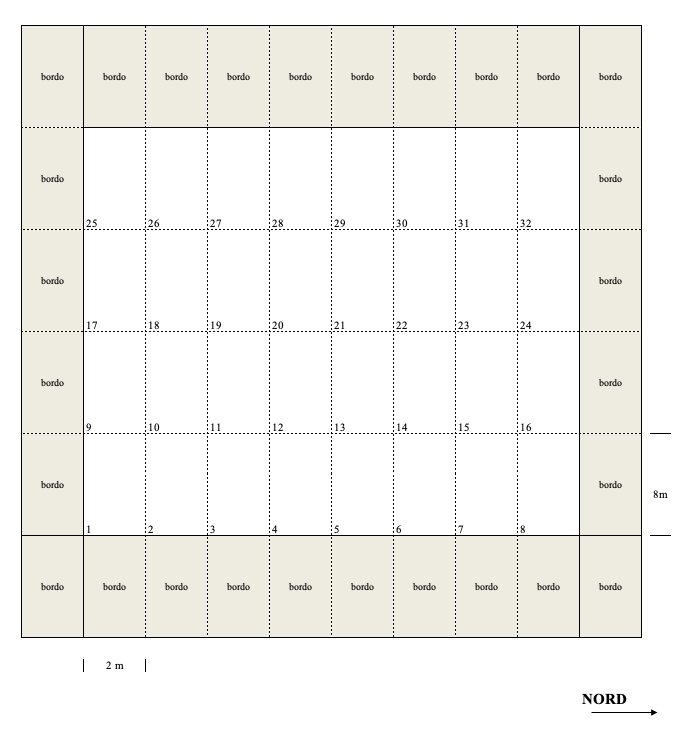
\includegraphics[width=0.9\linewidth]{_images/Mappa1} 

}

\caption{Mappa di campo di un esperimento con 32 parcelle}\label{fig:figName31}
\end{figure}

\hypertarget{allocazione-dei-trattamenti-e-disegno-sperimentale}{%
\section{Allocazione dei trattamenti e disegno sperimentale}\label{allocazione-dei-trattamenti-e-disegno-sperimentale}}

Il problema dell'allocazione dei trattamenti non si pone con gli esperimenti osservazionali, in quanto con questi si scelgono unità sperimentali già `naturalmente' trattate.

Per tutti gli esperimenti manipolati si pone invece il problema di scegliere quali soggetti trattare e come. A seconda di quali vincoli introduciamo nella selezioni dei soggetti possiamo avere diversi schemi sperimentali. Quelli che descriviamo di seguito, sono quelli più comunemente usati nella sperimentazione di pieno campo, ma, con le opportune modifiche, possono trovare impiego anche in molte altre discipline scientifiche.

\hypertarget{disegni-completamente-randomizzati}{%
\subsection{Disegni completamente randomizzati}\label{disegni-completamente-randomizzati}}

Per queste prove, le più semplici, la scelta dei soggetti da trattare è totalmente casuale, senza vincoli di sorta. Il vantaggio principale è la semplicità; lo svantaggio sta nel fatto che tutte le eventuali differenze e disomogeneità tra unità sperimentali restano non riconosciute ed entrano nella definizione della variabilità residua. Per questo, i disegno completamente randomizzati sono utilizzato soprattutto per le situazioni di buona uniformità ambientale e tra i soggetti.

Come esempio mostriamo un disegno completamente randomizzato utilizzando le parcelle della figura \ref{fig:figName31}, dove abbiamo allocato 8 trattamenti) identificati con le lettere da A ad H) con quattro repliche. Come si può notare, l'allocazione è completamente casuale (figura \ref{fig:figName33})

\begin{figure}

{\centering 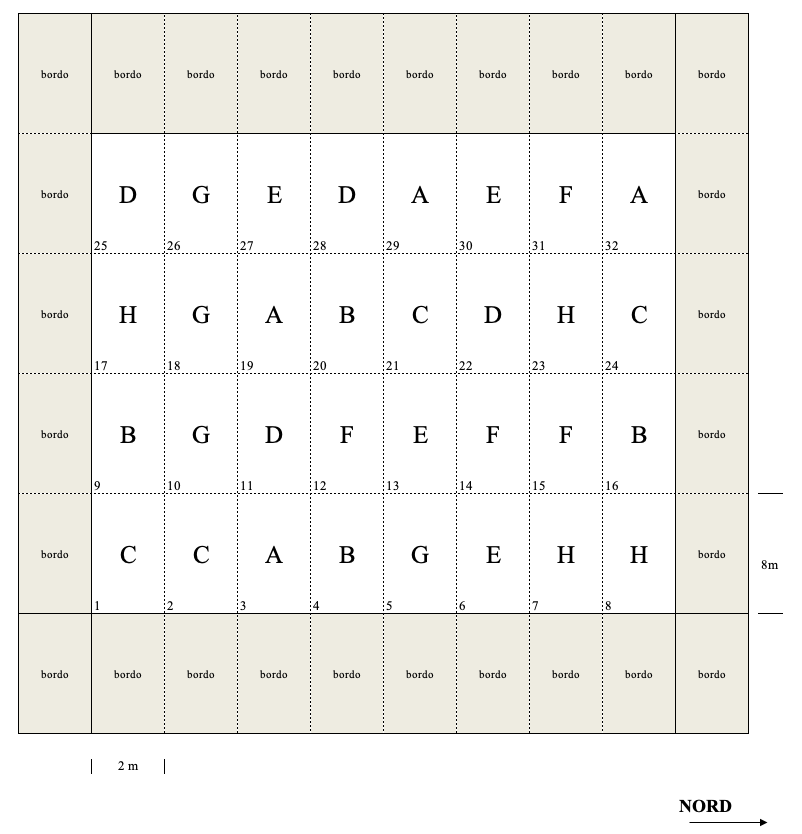
\includegraphics[width=0.9\linewidth]{_images/Mappa1CRD} 

}

\caption{Esempio di uno schema sperimentale a randomizzazione completa}\label{fig:figName33}
\end{figure}

\hypertarget{disegni-a-blocchi-randomizzati}{%
\subsection{Disegni a blocchi randomizzati}\label{disegni-a-blocchi-randomizzati}}

Quando le unità sperimentali non sono totalmenete omogenee, ma vi è una certa variabilità per una qualche caratteristiche rilevante, potremo dividere i soggetti in base a questa caratteristica, in tanti gruppi quante sono le repliche.

Ad esempio, nel caso dello schema in figura \ref{fig:figName31}, è lecito aspettarsi un gradiente trasversale, dato che il campo sarà certamente meno fertile vicino alle scoline. Per questo motivo, dato che abbiamo scelto di fare quattro repliche, divideremo l'appezzamento in quattro blocchi perpendicolari al gradiente di fertilità. Ad esempio il blocco 1 conterrà le parcelle 1, 9, 17, 25, 2, 10, 18 e 26, cioè le prime due colonne della mappa, con un numero di parcelle esattamente uguali al numero delle tesi. Il blocco 2 conterrà le colonne 3 e 4 e così via. Dato che il gradiente è trasversale, le parcelle di un stesso blocco saranno più omogenee che non parcelle su blocchi diversi. Dopo aver diviso la mappa in quattro blocchi di otto parcelle, possiamo allocare gli otto trattamenti a random all'interno di ogni blocco (\ref{fig:figName34})

\begin{figure}

{\centering 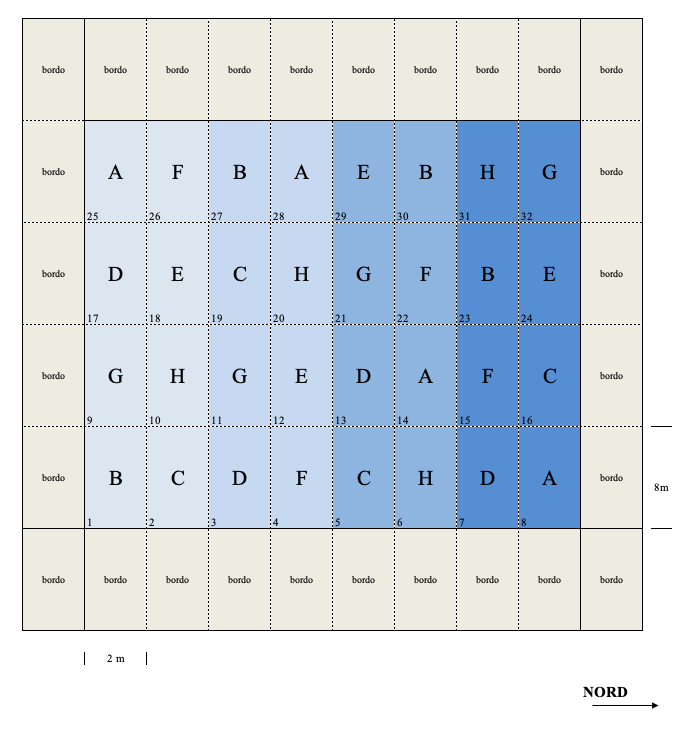
\includegraphics[width=0.9\linewidth]{_images/Mappa1CRBD} 

}

\caption{Esempio di uno schema sperimentale a blocchi randomizzati}\label{fig:figName34}
\end{figure}

Un disegno a blocchi randomizzati non è solo tipico della sperimentazione di campo. Ad esempio, volendo determinare la contaminazione da micotossine nelle confezioni di datteri, a seconda della modalità di confezionamento (es. carta, busta di plastica, scatola di plastica perforata), si può sospettare che il supermercato nel quale le confezioni vengono vendute potrebbe avere un certo effetto, legato alle modalità di conservazione. Per cui, invece che prelevare trenta confezioni (dieci per metodo) a caso nei supermercati di una città, scegliamo dieci supermercati e, in ognuno, prendiamo una confezione per tipo. In questo caso, il supermercato fa da blocco.

In generale, potremmo immaginare un esperimento con trattamenti che vengono allocati a caso agli animali di una stalla e ripetuti su stalle diverse, o a soggetti in gruppi omogenei di età e così via.

Il vantaggio del disegno a blocchi randomizzati sta nel fatto che ci permetto di utilizzare soggetti sperimentali con una più bassa omogeneità iniziale, aspetto importante quando il numero di unità sperimentali richieste comincia ad essere elevato. Infatti, le differenze tra soggetti sperimentali, almeno in parte, possono essere spiegate attraverso l'appartenenza ad un determinato gruppo e possono quindi essere scorporate dal calcolo della variabilità residua.

\hypertarget{disegni-a-quadrato-latino}{%
\subsection{Disegni a quadrato latino}\label{disegni-a-quadrato-latino}}

In questo caso, le unità sperimentali presentano due `gradienti', cioè vi sono differenze legate a due elementi importanti, oltre al trattamento sperimentale. Vediamo un esempio.

Una certo oggetto richiede un solo operatore per essere costruito, ma l'operazione può essere eseguita in quattro modi diversi. Vogliamo capire qual è il modo più veloce e, pertanto, pianifichiamo un esperimento. L'unità sperimentale è il lavoratore. I metodi sono quattro e, volendo lavorare con quattro repliche, avremmo bisogno di sedici operatori per disegnare un esperimento completamente randomizzato. Possiamo tuttavia considerare che un operatore, in quattro turni successivi, può operare con tutti e quattro i metodi. Quindi possiamo disegnare un esperimento in cui il turno fa da unità sperimentale e l'operatore fa da blocco (esperimento a blocchi randomizzati).

Tuttavia, in ogni blocco (operatore) vi è un gradiente, nel senso che i turni successivi al primo sono via via meno efficienti, perché l'operatore accumula stanchezza. Per tener conto di questo potremmo lasciare all'operatore un congruo periodo di tempo tra un turno e l'altro. Oppure, potremmo introdurre un vincolo ulteriore, per ogni operatore, randomizzando i quattro metodi tra i turni, in modo che ogni metodo, in operatori diversi, capiti in tutti i turni. In sostanza, l'operatore fa da blocco, perché in esso sono contenuti tutti i metodi. Ma anche il turno (per tutti gli operatori) fa da blocco, in quanto in esso sono ancora contenuti tutti i metodi. Proviamo a schematizzare, nella figura seguente (\ref{fig:figName391} ).

\begin{figure}

{\centering 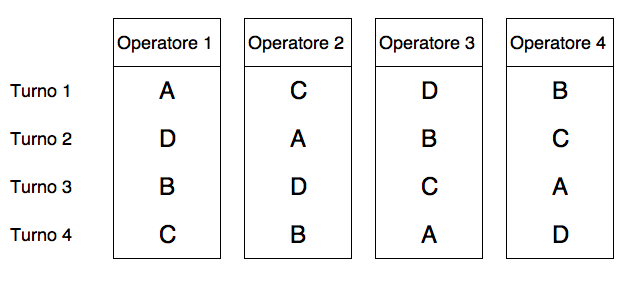
\includegraphics[width=0.9\linewidth]{_images/TurniOperatori} 

}

\caption{Allocazione di quattro metodi di lavoro (A, B, C e D), tra quattro operatori, in quattro turni, seguendo uno schema a quadrato latino}\label{fig:figName391}
\end{figure}

Questo schema prende il nome di quadrato latino, in quanto il numero delle repliche è uguale al numero dei trattamenti e, schematizzando lo schema su una mappa, otteniamo una griglia quadrata, nella quale ogni trattamento occupa tutte le righe e tutte le colonne. Chi lo conosce, riconosce in questo schema i principi di fondo del Sudoku.

Questo disegno è utile, perché possiamo dar conto sia delle differenza tra righe (turni), che delle differenze tra colonne (operatori), in modo da ridurre al minimo possibile la variabilità inspiegata. Lo svantaggio sta nel fatto che, dovendo avere tante repliche quanti sono i trattamenti, è utilizzabile solo per esperimenti abbastanza piccoli.

\textbf{{[}NOTA: Secondo me occorre inserire il disegno a split plot. Per ora non lo faccio per andare avanti e per decidere come vogliamo trattarlo. Metteresti i mixed in un corso magistrale?. Facendo una teoria leggera, secondo me si può fare, anche perchè introduce il concetto delle misure ripetute. Cosa facciamo?{]}}

\hypertarget{le-variabili-sperimentali}{%
\section{Le variabili sperimentali}\label{le-variabili-sperimentali}}

Per ogni singolo carattere, l'insieme delle modalità/valori che ognuno dei soggetti presenta prende il nome di \textbf{variabile} (proprio perché varia, cioè assume diversi valori, a seconda del soggetto).

Fondamentalmente, esistono due grandi gruppi di variabili: quelle che definiscono lo `stimolo' sperimentale e quelle che misurano la risposta dei soggetti trattati. Delle prime abbiamo già parlato, in quanto sono definite all'inizio dell'esperimento e rappresentano i livelli del/dei trattamento/i sperimentali. Ad esempio, fanno parte del primo gruppo le variabili come le modalità di lavorazione del suolo (aratura, minima lavorazione, semina su sodo) o il valore di azoto apportato (0, 50, 100, 150 kg N ha\textsuperscript{-1}). Le variabili che definiscono uno `stimolo' sperimentale sono anche dette variabili `indipendenti' in quanto non dipendono da nessun altro interno all'esperimento, a parte la volontà dello sperimentatore.

Durante e al termine dell'esperimento vengono invece rilevate le variabili `risposta' che esprimono l'effetto dei trattamenti sperimentali, come, ad esempio, la produzione della coltura, il peso delle piante trattate con un diserbante, la quantità di azoto lisciviato dopo la fertilizzazione. Queste variabili vengono normalmente definite `dipendenti', in quanto i valori assunti da ogni unità sperimentale dipendono, normalmente' dallo stimolo che hanno ricevuto.

Sia le variabili indipendenti sia quelle dipendenti possono essere di diversi tipi, che è molto importante saper riconoscere, perché condizionano il tipo di analisi statistica da eseguire. In particolare, distinguiamo:

\begin{enumerate}
\def\labelenumi{\arabic{enumi}.}
\tightlist
\item
  variabili nominali (categoriche);
\item
  variabili ordinali;
\item
  variabili quantitative discrete;
\item
  variabili quantitative continue.
\end{enumerate}

\hypertarget{variabili-nominali-categoriche}{%
\subsection{Variabili nominali (categoriche)}\label{variabili-nominali-categoriche}}

Le variabili nominali esprimono, per ciascun soggetto, l'appartenenza ad una determinata categoria o raggruppamento ed il valore che assumono lo definiamo modalità. L'unica caratteristica delle categorie è l'esclusività, cioè un soggetto che appartiene ad una di esse non può appartenere a nessuna delle altre. Variabili nominali sono, ad esempio, il sesso, la varietà, il tipo di diserbante impiegato, la lavorazione e così via. Le variabili categoriche permettono di raggruppare i soggetti, ma non possono essere utilizzate per fare calcoli, se non per definire le frequenze dei soggetti in ciascun gruppo.

\hypertarget{variabili-ordinali}{%
\subsection{Variabili ordinali}\label{variabili-ordinali}}

Anche le variabili ordinali esprimono, per ciascun soggetto, l'appartenenza ad una determinata categoria o raggruppamento. Tuttavia, le diverse categorie sono caratterizzate, oltre che dall'esclusività, anche da una relazione di ordine, nel senso che è possibile stabilire una naturale graduatoria tra esse. Ad esempio, la risposta degli agricoltori a domande relative alla loro percezione sull'utilità di una pratica agronomica può essere espressa utilizzando una scala con sei categorie (0, 1, 2, 3, 4 e 5), in ordine crescente da 0 a 5 (scala Likert). Di conseguenza possiamo confrontare categorie diverse ed esprimere un giudizio di ordine (2 è maggiore di 1, 3 è minore di 5), ma non possiamo eseguire operazioni matematiche, tipo sottrarre dalla categoria 3 la categoria 2 e così via, dato che la distanza tra le categorie non è necessariamente la stessa.

\hypertarget{variabili-quantitative-discrete}{%
\subsection{Variabili quantitative discrete}\label{variabili-quantitative-discrete}}

Le variabili discrete sono caratterizzate dal fatto che possiedono, oltre alle proprietà dell'esclusività e dell'ordine, anche quella dell'equidistanza tra gli attributi (es., in una scala a 5 punti, la distanza -- o la differenza -- fra 1 e 3 è uguale a quella fra 2 e 4 e doppia di quella tra 1 e 2). Una tipica variabile discreta è il conteggio di piante infestanti all'interno di una parcella di terreno.

Le variabili discrete consentono la gran parte delle operazioni matematiche e permettono di calcolare molte importanti statistiche come la media, la mediana, la varianza e la deviazione standard.

\hypertarget{variabili-quantitative-continue}{%
\subsection{Variabili quantitative continue}\label{variabili-quantitative-continue}}

Le variabili quantitative continue possiedono tutte le proprietà precedentemente esposte (esclusività delle categorie, ordine, distanza) oltre alla continuità, almeno in un certo intervallo. Tipiche variabili continue sono l'altezza, la produzione, il tempo, la fittezza\ldots{}

Dato che gli strumenti di misura nella realtà sono caratterizzati da una certa risoluzione, si potrebbe arguire che misure su scala continua effettivamente non esistono. Tuttavia questo argomento è più teorico che pratico e, nella ricerca biologica, consideriamo continue tutte le misure nelle quali la risoluzione dello strumento è sufficientemente piccola rispetto alla grandezza da misurare, purchè la scelta dello strumento sia effettuata in modo oculato. Viceversa, le variabili continue sono piuttosto rare nelle scienze economiche e sociali in genere.

La quantità di informazione fornita dagli strumenti di valutazione cresce passando dalle scale nominali, di più basso livello, a quelle quantitative continue, di livello più elevato. Variabili esprimibili con scale quantitative continue o discrete possono essere espresse anche con scale qualitative, adottando un'opportuna operazione di classamento. Il contrario, cioè trasformare in quantitativa una variabile qualitativa, non è invece possibile.
Va tuttavia ricordato che che le variabili discrete tendono ad assumere un comportamento simile alle continue quando il numero di valori che può essere assunto dalla variabile risulta molto ampio.

\hypertarget{rilievi-visivi-e-sensoriali}{%
\subsection{Rilievi visivi e sensoriali}\label{rilievi-visivi-e-sensoriali}}

Nella pratica sperimentale è molto frequente l'adozione di metodi di rilievo basati sull'osservazione di un fenomeno attraverso uno dei sensi (più spesso, la vista, ma anche gusto e olfatto) e l'assegnazione di una valutazione su scala categorica, ordinale o, con un po' di prudenza, quantitativa discreta o continua. Ad esempio, il ricoprimento delle piante infestanti, la percentuale di controllo di un erbicida e la sua fitotossicità vengono spesso rilevati visivamente, su scale da 0 a 100 o simili.

I vantaggi di questa tecnica sono molteplici:

\begin{enumerate}
\def\labelenumi{\arabic{enumi}.}
\tightlist
\item
  Basso costo ed elevata velocità
\item
  Possibilità di tener conto di alcuni fattori perturbativi esterni, che sono esclusi dalla valutazione, contrariamente a quello che succede con metodi oggettivi di misura
\item
  non richiede strumentazione costosa
\end{enumerate}

A questi vantaggi fanno da contraltare alcuni svantaggi, cioè:

\begin{enumerate}
\def\labelenumi{\arabic{enumi}.}
\tightlist
\item
  Minor precisione (in generale)
\item
  Soggettività
\item
  L'osservatore può essere prevenuto
\item
  Difficoltà di mantenere uniformità di giudizio
\item
  Richiede esperienza specifica e allenamento
\end{enumerate}

I rilievi sensoriali sono ben accettati nella pratica scientifica in alcuni ambiti ben definiti, anche se richiedono attenzione nell'analisi dei dati non potendo essere assimilati \emph{tout court} con le misure oggettive su scala continua.

\hypertarget{variabili-di-confondimento}{%
\subsection{Variabili di confondimento}\label{variabili-di-confondimento}}

Quando si pianificano i rilievi da eseguire, oppure anche nel corso dell'esecuzione di un esperimento, bisogna tener presente non soltanto la variabile che esprime l'effetto del trattamento, ma anche tutte le variabili che misurano possibili fattori di confondimento.

Ad esempio, immaginiamo di voler valutare la produttività di una specie arborea in funzione della varietà. Immaginiamo anche di sapere che, per questa specie, la produttività dipende anche dall'età. Se facciamo un esperimento possiamo utilizzare alberi della stessa età per minimizzare la variabilità dei soggetti. Tuttavia, se questo non fosse possibile, per ogni albero dobbiamo rilevare non solo la produttività, ma anche l'età, in modo da poter valutare anche l'effetto di questo fattore aggiuntivo e separarlo dall'effetto della varietà. In questo modo l'esperimento diviene molto più preciso.

\hypertarget{impianto-delle-prove}{%
\section{Impianto delle prove}\label{impianto-delle-prove}}

Da questo punto in poi, subentrano le competenze agronomiche e fitopatologiche necessarie per condurre gli esperimenti. Occorre, tuttavia, ricordare alcune pratiche usuali nella sperimentazione di pieno campo, destinate a migliorare l'efficienza della prova.

\begin{enumerate}
\def\labelenumi{\arabic{enumi}.}
\tightlist
\item
  Seminare a densità più alte e poi diradare, per assicurare una migliore uniformità di impianto
\item
  Prelevare da ogni parcella più campioni ed, eventualmente, omogeneizzarli o mediare i risultati ottenuti (vedi il caso dei 1000 semi)
\item
  Considerare le caratteristiche naturalmente meno variabili (es. la produzione areica e non la produzione per pianta)
\end{enumerate}

Si vuole inoltre ricordare che gli esperimenti parcellari configurano una situazione nella quale, per l'elevata cura che si pone nelle tecniche agronomiche, la produttività è almeno del 20\% superiore rispetto a quanto avviene nella normale pratica agricola.

\hypertarget{scrivere-un-progettoreport-di-ricerca-semplici-indicazioni}{%
\section{Scrivere un progetto/report di ricerca: semplici indicazioni}\label{scrivere-un-progettoreport-di-ricerca-semplici-indicazioni}}

Quanto abbiamo finora esposto costituisce uno schema generale che può essere adottato per redigere un progetto di ricerca o un report sui risultati ottenuti (tesi, pubblicazione). Bisogna provare che la ricerca che si è eseguita è precisa, accurata e replicabile/riproducibile e, di conseguenza, i risultati sono validi.

Nella redazione di un progetto di ricerca o di un report, è fondamentale tratteggiare bene i seguenti elementi:

\begin{enumerate}
\def\labelenumi{\arabic{enumi}.}
\tightlist
\item
  Titolo della ricerca
\item
  Descrizione del problema e background scientifico
\item
  Ipotesi scientifica, motivazioni e obiettivi
\item
  Tipo di esperimento e durata
\item
  Disegno sperimentale: trattamenti sperimentali (tesi) a confronto con dettagli relativi all'applicazione
\item
  Unità sperimentali e criteri per la loro selezione. Dettagli su repliche e randomizzazione
\item
  Dettagli su eventuali tecniche di `blocking'
\item
  Variabili da rilevare/rilevate
\item
  Dettagli su come le variabili saranno/sono state rilevate
\item
  Esposizione dei risultati (solo nel report)
\item
  Discussione (solo nel report)
\item
  Conclusioni (solo nel report)
\end{enumerate}

Alcuni aspetti che divengono elemento di valutazione del progetto e/o del report sono i seguenti:

\begin{enumerate}
\def\labelenumi{\arabic{enumi}.}
\tightlist
\item
  La selezione dei metodi deve essere coerente con gli obiettivi
\item
  Descrizione dettagliata dei materiali e metodi (bisogna che chiunque sia in grado di replicare l'esperimento)
\item
  Esposizione dei risultati chiara e convincente
\item
  Discussione approfondita e con molti riferimenti alla letteratura per confermare quanto ottenuto in passato o giusitificare risultati differenti.
\end{enumerate}

\begin{center}\rule{0.5\linewidth}{\linethickness}\end{center}

\hypertarget{per-approfondire-un-po-1}{%
\section{Per approfondire un po'\ldots{}}\label{per-approfondire-un-po-1}}

\hypertarget{esperimento-cieco-e-doppio-cieco}{%
\subsection{Esperimento `cieco' e `doppio cieco'}\label{esperimento-cieco-e-doppio-cieco}}

Per concludere questa parte, è opportuno menzionare il fatto che, in un esperimento scientifico, il fatto che lo sperimentatore e il soggetto siano coscienti del trattamento somministrato può portare a risultati distorti. Per esempio, nell'eseguire un rilievo, lo sperimentatore può essere influenzato dal sapere con quale diserbante è stata trattata una parcella, cercando inconsciamente conferme alle sue conoscenze pregresse. D'altro canto, nei soggetti sperimentali dotati di coscienza (uomo) sapere di essere stati trattati può influenzare l'esito del trattamento (effetto placebo).

Per evitare questi problemi, soprattutto in ambito medico, un esperimento può essere pianificato come:

\begin{enumerate}
\def\labelenumi{\arabic{enumi}.}
\tightlist
\item
  cieco: l'unità sperimentale o lo sperimentatore non sono coscienti dei dettagli del trattamento;
\item
  doppio cieco: né l'unità sperimentale né lo sperimentatore sono a coscienza dei dettagli del trattamento
\end{enumerate}

Un esperimento cieco e/o doppio cieco possono non essere eticamente corretti oppure inutili, nel qual caso si torna ad un esperimento tradizionale `aperto' (\emph{open experiment}: Tutti sanno tutto')

\begin{enumerate}
\def\labelenumi{\arabic{enumi}.}
\tightlist
\item
  Cochran, W.G., Cox, G.M., 1950. Experimental design. John Wiley \& Sons, Inc., Books.
\item
  LeClerg, E.L., Leonard, W.H., Clark, A.G., 1962. Field Plot Technique. Burgess Publishing Company, Books.
\end{enumerate}

\hypertarget{modelli-matematici-ed-analisi-dei-dati}{%
\chapter{Modelli matematici ed analisi dei dati}\label{modelli-matematici-ed-analisi-dei-dati}}

Placeholder

\hypertarget{verita-vera-e-modelli-deterministici}{%
\section{Verità `vera' e modelli deterministici}\label{verita-vera-e-modelli-deterministici}}

\hypertarget{qualche-esempio-di-modello-deterministico}{%
\subsection{Qualche esempio di modello deterministico}\label{qualche-esempio-di-modello-deterministico}}

\hypertarget{genesi-deterministica-delle-osservazioni-sperimentali}{%
\section{Genesi deterministica delle osservazioni sperimentali}\label{genesi-deterministica-delle-osservazioni-sperimentali}}

\hypertarget{errore-sperimentale-e-modelli-stocastici}{%
\section{Errore sperimentale e modelli stocastici}\label{errore-sperimentale-e-modelli-stocastici}}

\hypertarget{funzioni-di-probabilita}{%
\subsection{Funzioni di probabilità}\label{funzioni-di-probabilita}}

\hypertarget{funzioni-di-densita}{%
\subsection{Funzioni di densità}\label{funzioni-di-densita}}

\hypertarget{la-distribuzione-normale-curva-di-gauss}{%
\section{La distribuzione normale (curva di Gauss)}\label{la-distribuzione-normale-curva-di-gauss}}

\hypertarget{modelli-a-due-facce}{%
\section{Modelli `a due facce'}\label{modelli-a-due-facce}}

\hypertarget{e-allora}{%
\section{E allora?}\label{e-allora}}

\hypertarget{le-simulazioni-monte-carlo}{%
\section{Le simulazioni Monte Carlo}\label{le-simulazioni-monte-carlo}}

\hypertarget{analisi-dei-dati-e-model-fitting}{%
\section{Analisi dei dati e `model fitting'}\label{analisi-dei-dati-e-model-fitting}}

\hypertarget{per-approfondire-un-po-2}{%
\section{Per approfondire un po'\ldots{}}\label{per-approfondire-un-po-2}}

\hypertarget{generazione-dei-dati-sperimentali-un-esempio-piu-realistico}{%
\subsection{Generazione dei dati sperimentali: un esempio più realistico}\label{generazione-dei-dati-sperimentali-un-esempio-piu-realistico}}

\hypertarget{modelli-stocastici-non-normali}{%
\subsection{Modelli stocastici non-normali}\label{modelli-stocastici-non-normali}}

\hypertarget{t-di-student}{%
\subsubsection{t di Student}\label{t-di-student}}

\hypertarget{f-di-fisher}{%
\subsubsection{F di Fisher}\label{f-di-fisher}}

\hypertarget{la-distribuzione-binomiale}{%
\subsubsection{La distribuzione binomiale}\label{la-distribuzione-binomiale}}

\hypertarget{altre-letture}{%
\subsection{Altre letture}\label{altre-letture}}

\hypertarget{stime-ed-incertezza}{%
\chapter{Stime ed incertezza}\label{stime-ed-incertezza}}

Placeholder

\hypertarget{lanalisi-dei-dati-gli-ingredienti-fondamentali}{%
\section{L'analisi dei dati: gli `ingredienti' fondamentali}\label{lanalisi-dei-dati-gli-ingredienti-fondamentali}}

\hypertarget{esempio-una-soluzione-erbicida}{%
\section{Esempio: una soluzione erbicida}\label{esempio-una-soluzione-erbicida}}

\hypertarget{il-modello-dei-dati}{%
\subsection{Il modello dei dati}\label{il-modello-dei-dati}}

\hypertarget{analisi-dei-dati-stima-dei-parametri}{%
\subsection{Analisi dei dati: stima dei parametri}\label{analisi-dei-dati-stima-dei-parametri}}

\hypertarget{la-sampling-distribution}{%
\subsection{La `sampling distribution'}\label{la-sampling-distribution}}

\hypertarget{lerrore-standard}{%
\subsection{L'errore standard}\label{lerrore-standard}}

\hypertarget{riepilogo-1-caratterizzare-lincertezza-di-un-esperimento}{%
\section{Riepilogo 1: Caratterizzare l'incertezza di un esperimento}\label{riepilogo-1-caratterizzare-lincertezza-di-un-esperimento}}

\hypertarget{lintervallo-di-confidenza}{%
\section{L'intervallo di confidenza}\label{lintervallo-di-confidenza}}

\hypertarget{qual-e-il-senso-dellintervallo-di-confidenza}{%
\section{Qual è il senso dell'intervallo di confidenza?}\label{qual-e-il-senso-dellintervallo-di-confidenza}}

\hypertarget{come-presentare-i-risultati-degli-esperimenti}{%
\section{Come presentare i risultati degli esperimenti}\label{come-presentare-i-risultati-degli-esperimenti}}

\hypertarget{alcune-precisazioni}{%
\section{Alcune precisazioni}\label{alcune-precisazioni}}

\hypertarget{campioni-numerosi-e-non}{%
\subsection{Campioni numerosi e non}\label{campioni-numerosi-e-non}}

\hypertarget{popolazioni-gaussiane-e-non}{%
\subsection{Popolazioni gaussiane e non}\label{popolazioni-gaussiane-e-non}}

\hypertarget{analisi-statistica-dei-dati-riassunto-del-percorso-logico}{%
\section{Analisi statistica dei dati: riassunto del percorso logico}\label{analisi-statistica-dei-dati-riassunto-del-percorso-logico}}

\hypertarget{da-ricordare}{%
\section{Da ricordare}\label{da-ricordare}}

\hypertarget{esercizi}{%
\section{Esercizi}\label{esercizi}}

\hypertarget{per-approfondire-un-po-3}{%
\section{Per approfondire un po'\ldots{}}\label{per-approfondire-un-po-3}}

\hypertarget{coverage-degli-intervalli-di-confidenza}{%
\section{\texorpdfstring{\emph{Coverage} degli intervalli di confidenza}{Coverage degli intervalli di confidenza}}\label{coverage-degli-intervalli-di-confidenza}}

\hypertarget{intervalli-di-confidenza-per-fenomeni-non-normali}{%
\subsection{Intervalli di confidenza per fenomeni non-normali}\label{intervalli-di-confidenza-per-fenomeni-non-normali}}

\hypertarget{altre-letture-1}{%
\subsection{Altre letture}\label{altre-letture-1}}

\hypertarget{decisioni-e-incertezza}{%
\chapter{Decisioni e incertezza}\label{decisioni-e-incertezza}}

Placeholder

\hypertarget{confronto-tra-una-media-osservata-e-una-media-teorica}{%
\section{Confronto tra una media osservata e una media teorica}\label{confronto-tra-una-media-osservata-e-una-media-teorica}}

\hypertarget{simulazione-monte-carlo}{%
\subsection{Simulazione Monte Carlo}\label{simulazione-monte-carlo}}

\hypertarget{soluzione-formale}{%
\subsection{Soluzione formale}\label{soluzione-formale}}

\hypertarget{interpretazione-del-p-level}{%
\subsection{Interpretazione del P-level}\label{interpretazione-del-p-level}}

\hypertarget{confronto-tra-due-medie-il-test-t-di-student}{%
\section{Confronto tra due medie: il test t di Student}\label{confronto-tra-due-medie-il-test-t-di-student}}

\hypertarget{confronto-tra-due-proporzioni-il-test-chi2}{%
\section{\texorpdfstring{Confronto tra due proporzioni: il test \(\chi^2\)}{Confronto tra due proporzioni: il test \textbackslash{}chi\^{}2}}\label{confronto-tra-due-proporzioni-il-test-chi2}}

\hypertarget{conclusioni-1}{%
\section{Conclusioni}\label{conclusioni-1}}

\hypertarget{riepilogo}{%
\section{Riepilogo}\label{riepilogo}}

\hypertarget{esercizi-1}{%
\section{Esercizi}\label{esercizi-1}}

\hypertarget{per-approfondire-un-po-4}{%
\section{Per approfondire un po'\ldots{}}\label{per-approfondire-un-po-4}}

\hypertarget{tipologie-alternative-di-test-t-di-student}{%
\subsection{Tipologie alternative di test t di Student}\label{tipologie-alternative-di-test-t-di-student}}

\hypertarget{simulazione-del-p-value-nel-test-dipotesi}{%
\subsection{Simulazione del P-value nel test d'ipotesi}\label{simulazione-del-p-value-nel-test-dipotesi}}

\hypertarget{altre-letture-2}{%
\subsection{Altre letture}\label{altre-letture-2}}

\hypertarget{modelli-anova-ad-una-via}{%
\chapter{Modelli ANOVA ad una via}\label{modelli-anova-ad-una-via}}

Placeholder

\hypertarget{caso-studio-confronto-tra-erbicidi-in-vaso}{%
\section{Caso-studio: confronto tra erbicidi in vaso}\label{caso-studio-confronto-tra-erbicidi-in-vaso}}

\hypertarget{descrizione-del-dataset}{%
\section{Descrizione del dataset}\label{descrizione-del-dataset}}

\hypertarget{definizione-di-un-modello-lineare}{%
\section{Definizione di un modello lineare}\label{definizione-di-un-modello-lineare}}

\hypertarget{parametrizzazione-del-modello}{%
\section{Parametrizzazione del modello}\label{parametrizzazione-del-modello}}

\hypertarget{vincolo-sul-trattamento}{%
\subsection{Vincolo sul trattamento}\label{vincolo-sul-trattamento}}

\hypertarget{vincolo-sulla-somma}{%
\subsection{Vincolo sulla somma}\label{vincolo-sulla-somma}}

\hypertarget{assunzioni-di-base}{%
\section{Assunzioni di base}\label{assunzioni-di-base}}

\hypertarget{stima-dei-parametri}{%
\section{Stima dei parametri}\label{stima-dei-parametri}}

\hypertarget{coefficienti-del-modello}{%
\subsection{Coefficienti del modello}\label{coefficienti-del-modello}}

\hypertarget{residui}{%
\subsection{Residui}\label{residui}}

\hypertarget{stima-di-sigma}{%
\subsection{\texorpdfstring{Stima di \(\sigma\)}{Stima di \textbackslash{}sigma}}\label{stima-di-sigma}}

\hypertarget{sem-e-sed}{%
\subsection{SEM e SED}\label{sem-e-sed}}

\hypertarget{scomposizione-della-varianza}{%
\section{Scomposizione della varianza}\label{scomposizione-della-varianza}}

\hypertarget{test-dipotesi}{%
\section{Test d'ipotesi}\label{test-dipotesi}}

\hypertarget{operazioni-con-r}{%
\section{Operazioni con R}\label{operazioni-con-r}}

\hypertarget{medie-marginali-attese}{%
\section{Medie marginali attese}\label{medie-marginali-attese}}

\hypertarget{per-concludere}{%
\section{Per concludere \ldots{}}\label{per-concludere}}

\hypertarget{per-approfondire-un-po-5}{%
\section{Per approfondire un po'\ldots{}}\label{per-approfondire-un-po-5}}

\hypertarget{simulazione-della-sampling-distribution-per-f}{%
\subsection{\texorpdfstring{Simulazione della \emph{sampling distribution} per F}{Simulazione della sampling distribution per F}}\label{simulazione-della-sampling-distribution-per-f}}

\hypertarget{altre-letture-3}{%
\subsection{Altre letture}\label{altre-letture-3}}

\hypertarget{la-verifica-delle-assunzioni-di-base}{%
\chapter{La verifica delle assunzioni di base}\label{la-verifica-delle-assunzioni-di-base}}

Placeholder

\hypertarget{procedure-diagnostiche}{%
\section{Procedure diagnostiche}\label{procedure-diagnostiche}}

\hypertarget{analisi-grafica-dei-residui}{%
\section{Analisi grafica dei residui}\label{analisi-grafica-dei-residui}}

\hypertarget{grafico-dei-residui-contro-i-valori-attesi}{%
\subsection{Grafico dei residui contro i valori attesi}\label{grafico-dei-residui-contro-i-valori-attesi}}

\hypertarget{qq-plot}{%
\subsection{QQ-plot}\label{qq-plot}}

\hypertarget{strumenti-diagnostici-formali}{%
\section{Strumenti diagnostici formali}\label{strumenti-diagnostici-formali}}

\hypertarget{risultati-contraddittori}{%
\section{Risultati contraddittori}\label{risultati-contraddittori}}

\hypertarget{terapia}{%
\section{`Terapia'}\label{terapia}}

\hypertarget{correzionerimozione-degli-outliers}{%
\subsection{Correzione/Rimozione degli outliers}\label{correzionerimozione-degli-outliers}}

\hypertarget{correzione-del-modello}{%
\subsection{Correzione del modello}\label{correzione-del-modello}}

\hypertarget{trasformazione-della-variabile-indipendente}{%
\subsection{Trasformazione della variabile indipendente}\label{trasformazione-della-variabile-indipendente}}

\hypertarget{impiego-di-metodiche-statistiche-avanzate}{%
\subsection{Impiego di metodiche statistiche avanzate}\label{impiego-di-metodiche-statistiche-avanzate}}

\hypertarget{trasformazioni-stabilizzanti}{%
\subsection{Trasformazioni stabilizzanti}\label{trasformazioni-stabilizzanti}}

\hypertarget{esempio}{%
\section{Esempio}\label{esempio}}

\hypertarget{per-approfondire-un-po-6}{%
\section{Per approfondire un po' \ldots{}}\label{per-approfondire-un-po-6}}

\hypertarget{contrasti-e-confronti-multipli}{%
\chapter{Contrasti e confronti multipli}\label{contrasti-e-confronti-multipli}}

Placeholder

\hypertarget{esempio-1}{%
\section{Esempio}\label{esempio-1}}

\hypertarget{i-contrasti}{%
\section{I contrasti}\label{i-contrasti}}

\hypertarget{varianza-del-contrasto-e-test-dipotesi}{%
\subsection{Varianza del contrasto e test d'ipotesi}\label{varianza-del-contrasto-e-test-dipotesi}}

\hypertarget{i-contrasti-con-r}{%
\subsection{I contrasti con R}\label{i-contrasti-con-r}}

\hypertarget{i-confronti-multipli-a-coppie-pairwise-comparisons}{%
\section{I confronti multipli a coppie (pairwise comparisons)}\label{i-confronti-multipli-a-coppie-pairwise-comparisons}}

\hypertarget{display-a-lettere}{%
\section{Display a lettere}\label{display-a-lettere}}

\hypertarget{problemi-di-molteplicita-tassi-di-errore-per-confronto-e-per-esperimento}{%
\section{Problemi di molteplicità: tassi di errore per confronto e per esperimento}\label{problemi-di-molteplicita-tassi-di-errore-per-confronto-e-per-esperimento}}

\hypertarget{correzione-per-la-molteplicita}{%
\subsection{Correzione per la molteplicità}\label{correzione-per-la-molteplicita}}

\hypertarget{e-le-classiche-procedure-di-confronto-multiplo}{%
\section{E le classiche procedure di confronto multiplo?}\label{e-le-classiche-procedure-di-confronto-multiplo}}

\hypertarget{consigli-pratici}{%
\section{Consigli pratici}\label{consigli-pratici}}

\hypertarget{per-approfondire-un-po-7}{%
\section{Per approfondire un po'\ldots{}}\label{per-approfondire-un-po-7}}

\hypertarget{intervallo-di-confidenza-di-un-contrasto}{%
\subsection{Intervallo di confidenza di un contrasto}\label{intervallo-di-confidenza-di-un-contrasto}}

\hypertarget{correzione-per-la-molteplicita-qualche-dettaglio-ulteriore}{%
\subsection{Correzione per la molteplicità: qualche dettaglio ulteriore}\label{correzione-per-la-molteplicita-qualche-dettaglio-ulteriore}}

\hypertarget{altre-letture-4}{%
\subsection{Altre letture}\label{altre-letture-4}}

\hypertarget{modelli-anova-con-fattori-di-blocco}{%
\chapter{Modelli ANOVA con fattori di blocco}\label{modelli-anova-con-fattori-di-blocco}}

Placeholder

\hypertarget{caso-studio-confronto-tra-erbicidi-in-campo}{%
\section{Caso-studio: confronto tra erbicidi in campo}\label{caso-studio-confronto-tra-erbicidi-in-campo}}

\hypertarget{definizione-di-un-modello-lineare-1}{%
\section{Definizione di un modello lineare}\label{definizione-di-un-modello-lineare-1}}

\hypertarget{stima-dei-parametri-1}{%
\section{Stima dei parametri}\label{stima-dei-parametri-1}}

\hypertarget{coefficienti-del-modello-1}{%
\subsection{Coefficienti del modello}\label{coefficienti-del-modello-1}}

\hypertarget{residui-e-devianze}{%
\subsection{Residui e devianze}\label{residui-e-devianze}}

\hypertarget{scomposizione-della-varianza-1}{%
\section{Scomposizione della varianza}\label{scomposizione-della-varianza-1}}

\hypertarget{disegni-a-quadrato-latino-1}{%
\section{Disegni a quadrato latino}\label{disegni-a-quadrato-latino-1}}

\hypertarget{caso-studio-confronto-tra-metodi-costruttivi}{%
\section{Caso studio: confronto tra metodi costruttivi}\label{caso-studio-confronto-tra-metodi-costruttivi}}

\hypertarget{definizione-di-un-modello-lineare-2}{%
\section{Definizione di un modello lineare}\label{definizione-di-un-modello-lineare-2}}

\hypertarget{modelli-anova-a-due-vie}{%
\chapter{Modelli ANOVA a due vie}\label{modelli-anova-a-due-vie}}

Placeholder

\hypertarget{il-concetto-di-interazione}{%
\section{Il concetto di 'interazione'}\label{il-concetto-di-interazione}}

\hypertarget{tipi-di-interazione}{%
\section{Tipi di interazione}\label{tipi-di-interazione}}

\hypertarget{caso-studio-interazione-tra-lavorazioni-e-diserbo-chimico}{%
\section{Caso-studio: interazione tra lavorazioni e diserbo chimico}\label{caso-studio-interazione-tra-lavorazioni-e-diserbo-chimico}}

\hypertarget{definizione-del-modello-lineare}{%
\section{Definizione del modello lineare}\label{definizione-del-modello-lineare}}

\hypertarget{stima-dei-parametri-2}{%
\section{Stima dei parametri}\label{stima-dei-parametri-2}}

\hypertarget{verifica-delle-assunzioni-di-base}{%
\section{Verifica delle assunzioni di base}\label{verifica-delle-assunzioni-di-base}}

\hypertarget{scomposizione-delle-varianze}{%
\section{Scomposizione delle varianze}\label{scomposizione-delle-varianze}}

\hypertarget{medie-marginali-attese-1}{%
\section{Medie marginali attese}\label{medie-marginali-attese-1}}

\hypertarget{calcolo-degli-errori-standard-sem-e-sed}{%
\section{Calcolo degli errori standard (SEM e SED)}\label{calcolo-degli-errori-standard-sem-e-sed}}

\hypertarget{medie-marginali-attese-e-confronti-multipli-con-r}{%
\section{Medie marginali attese e confronti multipli con R}\label{medie-marginali-attese-e-confronti-multipli-con-r}}

\hypertarget{per-approfondire-un-po.}{%
\section{Per approfondire un po'\ldots{}.}\label{per-approfondire-un-po.}}

\hypertarget{anova-a-due-vie-scomposizione-manuale-della-varianza}{%
\subsection{Anova a due vie: scomposizione `manuale' della varianza}\label{anova-a-due-vie-scomposizione-manuale-della-varianza}}

\hypertarget{la-regressione-lineare-semplice}{%
\chapter{La regressione lineare semplice}\label{la-regressione-lineare-semplice}}

Placeholder

\hypertarget{caso-studio-effetto-della-concimazione-azotata-al-frumento}{%
\section{Caso studio: effetto della concimazione azotata al frumento}\label{caso-studio-effetto-della-concimazione-azotata-al-frumento}}

\hypertarget{analisi-preliminari}{%
\section{Analisi preliminari}\label{analisi-preliminari}}

\hypertarget{definizione-del-modello-lineare-1}{%
\section{Definizione del modello lineare}\label{definizione-del-modello-lineare-1}}

\hypertarget{stima-dei-parametri-3}{%
\section{Stima dei parametri}\label{stima-dei-parametri-3}}

\hypertarget{valutazione-della-bonta-del-modello}{%
\section{Valutazione della bontà del modello}\label{valutazione-della-bonta-del-modello}}

\hypertarget{valutazione-grafica}{%
\subsection{Valutazione grafica}\label{valutazione-grafica}}

\hypertarget{errori-standard-dei-parametri}{%
\subsection{Errori standard dei parametri}\label{errori-standard-dei-parametri}}

\hypertarget{test-f-per-la-mancanza-dadattamento}{%
\subsection{Test F per la mancanza d'adattamento}\label{test-f-per-la-mancanza-dadattamento}}

\hypertarget{test-f-per-la-bonta-di-adattamento-e-coefficiente-di-determinazione}{%
\subsection{Test F per la bontà di adattamento e coefficiente di determinazione}\label{test-f-per-la-bonta-di-adattamento-e-coefficiente-di-determinazione}}

\hypertarget{previsioni}{%
\section{Previsioni}\label{previsioni}}

\hypertarget{per-approfondire-un-po-8}{%
\section{Per approfondire un po'\ldots{}}\label{per-approfondire-un-po-8}}

\hypertarget{la-regressione-non-lineare}{%
\chapter{La regressione non-lineare}\label{la-regressione-non-lineare}}

Placeholder

\hypertarget{caso-studio-degradazione-di-un-erbicida-nel-terreno}{%
\section{Caso studio: degradazione di un erbicida nel terreno}\label{caso-studio-degradazione-di-un-erbicida-nel-terreno}}

\hypertarget{scelta-della-funzione}{%
\section{Scelta della funzione}\label{scelta-della-funzione}}

\hypertarget{stima-dei-parametri-4}{%
\section{Stima dei parametri}\label{stima-dei-parametri-4}}

\hypertarget{linearizzazione-della-funzione}{%
\subsection{Linearizzazione della funzione}\label{linearizzazione-della-funzione}}

\hypertarget{approssimazione-della-vera-funzione-tramite-una-polinomiale-in-x}{%
\subsection{Approssimazione della vera funzione tramite una polinomiale in X}\label{approssimazione-della-vera-funzione-tramite-una-polinomiale-in-x}}

\hypertarget{minimi-quadrati-non-lineari}{%
\subsection{Minimi quadrati non-lineari}\label{minimi-quadrati-non-lineari}}

\hypertarget{la-regressione-non-lineare-con-r}{%
\section{La regressione non-lineare con R}\label{la-regressione-non-lineare-con-r}}

\hypertarget{verifica-della-bonta-del-modello}{%
\section{Verifica della bontà del modello}\label{verifica-della-bonta-del-modello}}

\hypertarget{analisi-grafica-dei-residui-1}{%
\subsection{Analisi grafica dei residui}\label{analisi-grafica-dei-residui-1}}

\hypertarget{test-f-per-la-mancanza-di-adattamento-approssimato}{%
\subsection{Test F per la mancanza di adattamento (approssimato)}\label{test-f-per-la-mancanza-di-adattamento-approssimato}}

\hypertarget{errori-standard-dei-parametri-1}{%
\subsection{Errori standard dei parametri}\label{errori-standard-dei-parametri-1}}

\hypertarget{coefficienti-di-determinazione}{%
\subsection{Coefficienti di determinazione}\label{coefficienti-di-determinazione}}

\hypertarget{funzioni-lineari-e-nonlineari-dei-parametri}{%
\section{Funzioni lineari e nonlineari dei parametri}\label{funzioni-lineari-e-nonlineari-dei-parametri}}

\hypertarget{previsioni-1}{%
\section{Previsioni}\label{previsioni-1}}

\hypertarget{gestione-delle-situazioni-patologiche}{%
\section{Gestione delle situazioni `patologiche'}\label{gestione-delle-situazioni-patologiche}}

\hypertarget{trasformazione-del-modello}{%
\subsection{Trasformazione del modello}\label{trasformazione-del-modello}}

\hypertarget{trasformazione-dei-dati}{%
\subsection{Trasformazione dei dati}\label{trasformazione-dei-dati}}

\hypertarget{per-approfondire-un-po-9}{%
\section{Per approfondire un po'\ldots{}}\label{per-approfondire-un-po-9}}

\hypertarget{riparametrizzazione-delle-funzioni-non-lineari}{%
\subsection{Riparametrizzazione delle funzioni non-lineari}\label{riparametrizzazione-delle-funzioni-non-lineari}}

\hypertarget{altre-letture-5}{%
\subsection{Altre letture}\label{altre-letture-5}}

\hypertarget{appendice-1-breve-introduzione-ad-r}{%
\chapter{Appendice 1: breve introduzione ad R}\label{appendice-1-breve-introduzione-ad-r}}

Placeholder

\hypertarget{cosa-e-r}{%
\section*{Cosa è R?}\label{cosa-e-r}}
\addcontentsline{toc}{section}{Cosa è R?}

\hypertarget{oggetti-e-assegnazioni}{%
\section*{Oggetti e assegnazioni}\label{oggetti-e-assegnazioni}}
\addcontentsline{toc}{section}{Oggetti e assegnazioni}

\hypertarget{costanti-e-vettori}{%
\subsection*{Costanti e vettori}\label{costanti-e-vettori}}
\addcontentsline{toc}{subsection}{Costanti e vettori}

\hypertarget{matrici}{%
\subsection*{Matrici}\label{matrici}}
\addcontentsline{toc}{subsection}{Matrici}

\hypertarget{dataframe}{%
\subsection*{Dataframe}\label{dataframe}}
\addcontentsline{toc}{subsection}{Dataframe}

\hypertarget{quale-oggetto-sto-utilizzando}{%
\subsection*{Quale oggetto sto utilizzando?}\label{quale-oggetto-sto-utilizzando}}
\addcontentsline{toc}{subsection}{Quale oggetto sto utilizzando?}

\hypertarget{operazioni-ed-operatori}{%
\section*{Operazioni ed operatori}\label{operazioni-ed-operatori}}
\addcontentsline{toc}{section}{Operazioni ed operatori}

\hypertarget{funzioni-ed-argomenti}{%
\section*{Funzioni ed argomenti}\label{funzioni-ed-argomenti}}
\addcontentsline{toc}{section}{Funzioni ed argomenti}

\hypertarget{consigli-per-limmissione-di-dati-sperimentali}{%
\section*{Consigli per l'immissione di dati sperimentali}\label{consigli-per-limmissione-di-dati-sperimentali}}
\addcontentsline{toc}{section}{Consigli per l'immissione di dati sperimentali}

\hypertarget{immissione-manuale-di-dati}{%
\subsection*{Immissione manuale di dati}\label{immissione-manuale-di-dati}}
\addcontentsline{toc}{subsection}{Immissione manuale di dati}

\hypertarget{immissione-di-numeri-progressivi}{%
\subsection*{Immissione di numeri progressivi}\label{immissione-di-numeri-progressivi}}
\addcontentsline{toc}{subsection}{Immissione di numeri progressivi}

\hypertarget{immissione-dei-codici-delle-tesi-e-dei-blocchi}{%
\subsection*{Immissione dei codici delle tesi e dei blocchi}\label{immissione-dei-codici-delle-tesi-e-dei-blocchi}}
\addcontentsline{toc}{subsection}{Immissione dei codici delle tesi e dei blocchi}

\hypertarget{leggere-e-salvare-dati-esterni}{%
\subsection*{Leggere e salvare dati esterni}\label{leggere-e-salvare-dati-esterni}}
\addcontentsline{toc}{subsection}{Leggere e salvare dati esterni}

\hypertarget{alcune-operazioni-comuni-sul-dataset}{%
\section*{Alcune operazioni comuni sul dataset}\label{alcune-operazioni-comuni-sul-dataset}}
\addcontentsline{toc}{section}{Alcune operazioni comuni sul dataset}

\hypertarget{selezionare-un-subset-di-dati}{%
\subsection*{Selezionare un subset di dati}\label{selezionare-un-subset-di-dati}}
\addcontentsline{toc}{subsection}{Selezionare un subset di dati}

\hypertarget{ordinare-un-vettore-o-un-dataframe}{%
\subsection*{Ordinare un vettore o un dataframe}\label{ordinare-un-vettore-o-un-dataframe}}
\addcontentsline{toc}{subsection}{Ordinare un vettore o un dataframe}

\hypertarget{workspace}{%
\section*{Workspace}\label{workspace}}
\addcontentsline{toc}{section}{Workspace}

\hypertarget{script-o-programmi}{%
\section*{Script o programmi}\label{script-o-programmi}}
\addcontentsline{toc}{section}{Script o programmi}

\hypertarget{interrogazione-di-oggetti}{%
\section*{Interrogazione di oggetti}\label{interrogazione-di-oggetti}}
\addcontentsline{toc}{section}{Interrogazione di oggetti}

\hypertarget{altre-funzioni-matriciali}{%
\section*{Altre funzioni matriciali}\label{altre-funzioni-matriciali}}
\addcontentsline{toc}{section}{Altre funzioni matriciali}

\hypertarget{cenni-sulle-funzionalita-grafiche-in-r}{%
\section*{Cenni sulle funzionalità grafiche in R}\label{cenni-sulle-funzionalita-grafiche-in-r}}
\addcontentsline{toc}{section}{Cenni sulle funzionalità grafiche in R}

\hypertarget{per-approfondire-un-po-10}{%
\section{Per approfondire un po'\ldots{}}\label{per-approfondire-un-po-10}}

\hypertarget{appendice-2-richiami-di-statistica-descrittiva}{%
\chapter{Appendice 2: Richiami di statistica descrittiva}\label{appendice-2-richiami-di-statistica-descrittiva}}

Placeholder

\hypertarget{dati-quantitativi-analisi-chimiche-e-altre-misurazioni-fondamentali}{%
\section*{Dati quantitativi: analisi chimiche e altre misurazioni fondamentali}\label{dati-quantitativi-analisi-chimiche-e-altre-misurazioni-fondamentali}}
\addcontentsline{toc}{section}{Dati quantitativi: analisi chimiche e altre misurazioni fondamentali}

\hypertarget{indicatori-di-tendenza-centrale}{%
\subsection*{Indicatori di tendenza centrale}\label{indicatori-di-tendenza-centrale}}
\addcontentsline{toc}{subsection}{Indicatori di tendenza centrale}

\hypertarget{indicatori-di-dispersione}{%
\subsection*{Indicatori di dispersione}\label{indicatori-di-dispersione}}
\addcontentsline{toc}{subsection}{Indicatori di dispersione}

\hypertarget{arrotondamenti}{%
\subsection*{Arrotondamenti}\label{arrotondamenti}}
\addcontentsline{toc}{subsection}{Arrotondamenti}

\hypertarget{descrizione-dei-sottogruppi}{%
\subsection*{Descrizione dei sottogruppi}\label{descrizione-dei-sottogruppi}}
\addcontentsline{toc}{subsection}{Descrizione dei sottogruppi}

\hypertarget{relazioni-tra-variabili-quantitative-correlazione}{%
\subsection{Relazioni tra variabili quantitative: correlazione}\label{relazioni-tra-variabili-quantitative-correlazione}}

\hypertarget{dati-qualitativi-conteggi-e-frequenze}{%
\section*{Dati qualitativi: conteggi e frequenze}\label{dati-qualitativi-conteggi-e-frequenze}}
\addcontentsline{toc}{section}{Dati qualitativi: conteggi e frequenze}

\hypertarget{distribuzioni-di-frequenze-e-classamento}{%
\subsection*{Distribuzioni di frequenze e classamento}\label{distribuzioni-di-frequenze-e-classamento}}
\addcontentsline{toc}{subsection}{Distribuzioni di frequenze e classamento}

\hypertarget{statistiche-descrittive-per-le-distribuzioni-di-frequenze}{%
\subsection*{Statistiche descrittive per le distribuzioni di frequenze}\label{statistiche-descrittive-per-le-distribuzioni-di-frequenze}}
\addcontentsline{toc}{subsection}{Statistiche descrittive per le distribuzioni di frequenze}

\hypertarget{distribuzioni-di-frequenza-bivariate-le-tabelle-di-contingenza}{%
\subsection*{Distribuzioni di frequenza bivariate: le tabelle di contingenza}\label{distribuzioni-di-frequenza-bivariate-le-tabelle-di-contingenza}}
\addcontentsline{toc}{subsection}{Distribuzioni di frequenza bivariate: le tabelle di contingenza}

\hypertarget{connessione}{%
\subsection*{Connessione}\label{connessione}}
\addcontentsline{toc}{subsection}{Connessione}

\hypertarget{esercizi-2}{%
\section*{Esercizi}\label{esercizi-2}}
\addcontentsline{toc}{section}{Esercizi}

\hypertarget{esercizio-1}{%
\subsection*{Esercizio 1}\label{esercizio-1}}
\addcontentsline{toc}{subsection}{Esercizio 1}

\hypertarget{esercizio-2}{%
\subsection*{Esercizio 2}\label{esercizio-2}}
\addcontentsline{toc}{subsection}{Esercizio 2}

\hypertarget{per-approfondire-un-po-11}{%
\section{Per approfondire un po'\ldots{}}\label{per-approfondire-un-po-11}}


\end{document}
